\section{ХОД РАБОТЫ}

\subsection{Постановка задачи}

На производственном участке имеются три автоматических станка:
два станка типа СТ1 и один станок типа СТ2.

Каждый станок оснащен бункером; у станков СТ1 бункер вмещает
20 заголовок для изготовления деталей, у станка СТ2 --- 30 заготовок.

Время, необходимое для обработки на станке одной заготовки --- случайная величина,
распределенная по гауссовскому закону, со средним значением 3 мин
и стандартным отклонением 20 с.

Станок обрабатывает все заготовки, имеющиеся в бункере.
После израсходования заготовок, находящихся в бункере,
необходимо заполнение бункера заготовками. После заполнения бункера станок возобновляет работу.

Заполнение бункеров заготовками выполняется оператором, обслуживающим станки.
Заполнение бункера станка СТ1 занимает у оператора от 10 до 20 мин,
станка СТ2 --- от 15 до 25 мин.

Требуется разработать GPSS-модель для анализа работы производственного участка
в течение 100 часов. Предусмотреть получение данных о времени простоя станков
(т.~е.~о времени от момента остановки станка из-за израсходования заготовок
до момента возобновления его работы) в табличной форме, причем требуется
получить две таблицы: для станков типа СТ1 и типа СТ2.
Предусмотреть вычисление простоя станков в процентах.


\subsection{Решение задачи}

Разработанная GPSS-модель представлена в приложении~А. После выполнения сеанса
моделирования исходной задачи, получим отчёт, представленные на
рисунках~\ref{pic:report_1}--\ref{pic:report_3}.

\newpage

\begin{figure}[h!]
  \centering
  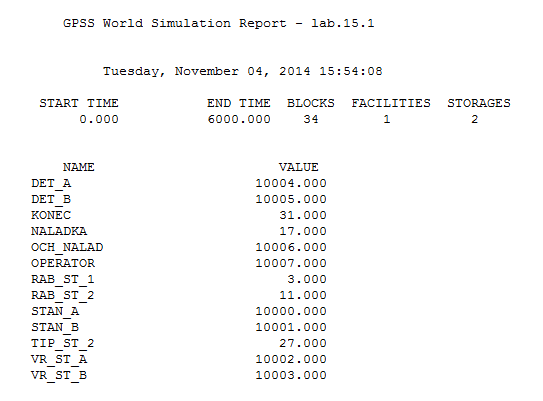
\includegraphics[width=1\linewidth]{pic/report_1}
  \caption{Выходные данные имитационной модели}
  \label{pic:report_1}
\end{figure}

\newpage

\begin{figure}[h!]
  \centering
  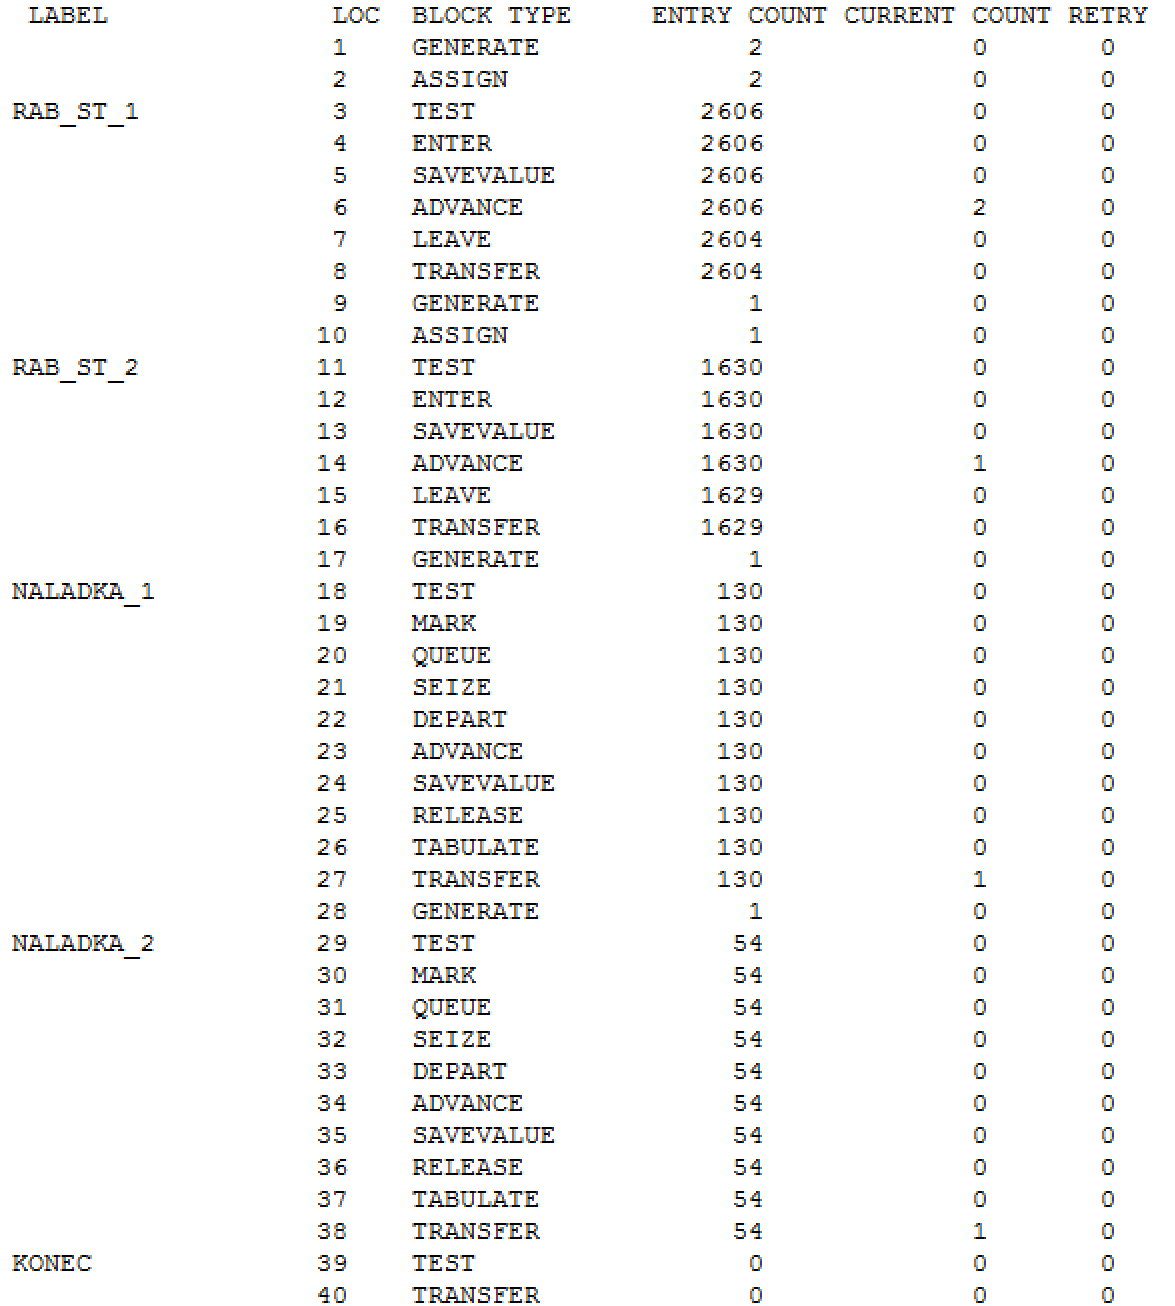
\includegraphics[width=1\linewidth]{pic/report_2}
  \caption{Статистика исполнения команд имитационной модели}
  \label{pic:report_2}
\end{figure}

\newpage

\begin{figure}[h!]
  \centering
  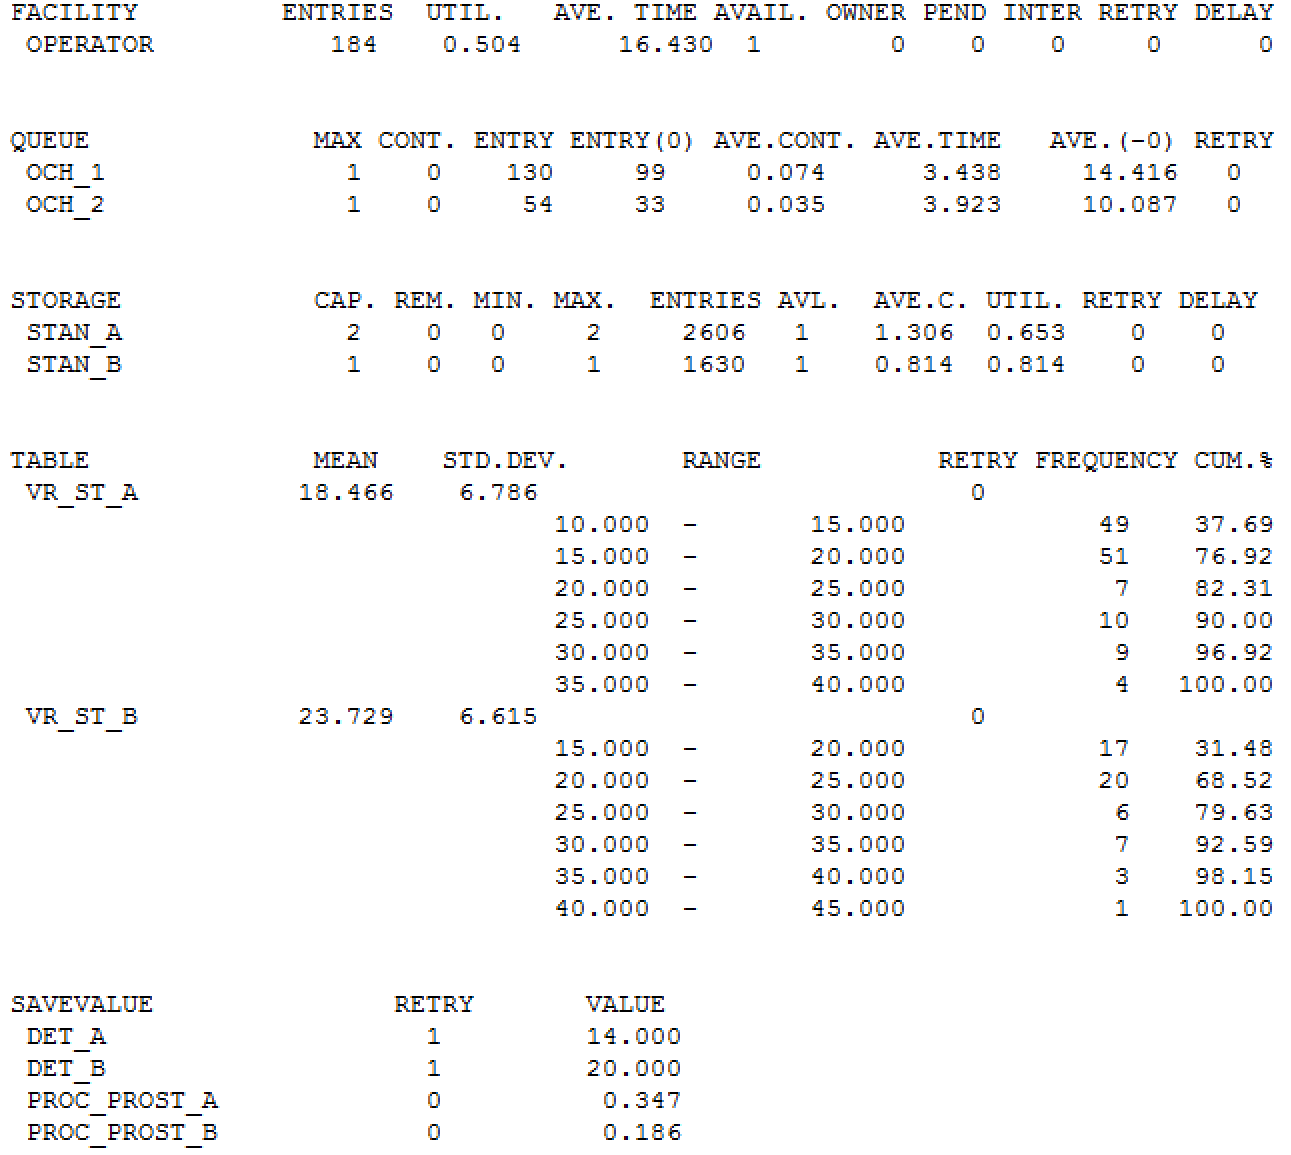
\includegraphics[width=0.8\linewidth]{pic/report_3}
  \caption{Статистика использования узлов моделируемой СМО}
  \label{pic:report_3}
\end{figure}

Среднее значеие простоя станков указано в таблицах VR\_ST\_A и VR\_ST\_B,
изображенных на рисунке~\ref{pic:report_3}. В результате моделирования получены
следующие значения:

\begin{itemize}
  \item среднее время простоя станка типа A --- 21{,}8~(мин);
  \item среднее время простоя станка типа B --- 29{,}8~(мин).
\end{itemize}

\newpage

На основе данных, полученных из таблиц VR\_ST\_A и VR\_ST\_B построим
гистограммы распределения времени простоя станков, представленные
на рисунках~\ref{pic:histogram_1}--\ref{pic:histogram_2}.

\begin{figure}[h!]
  \centering
  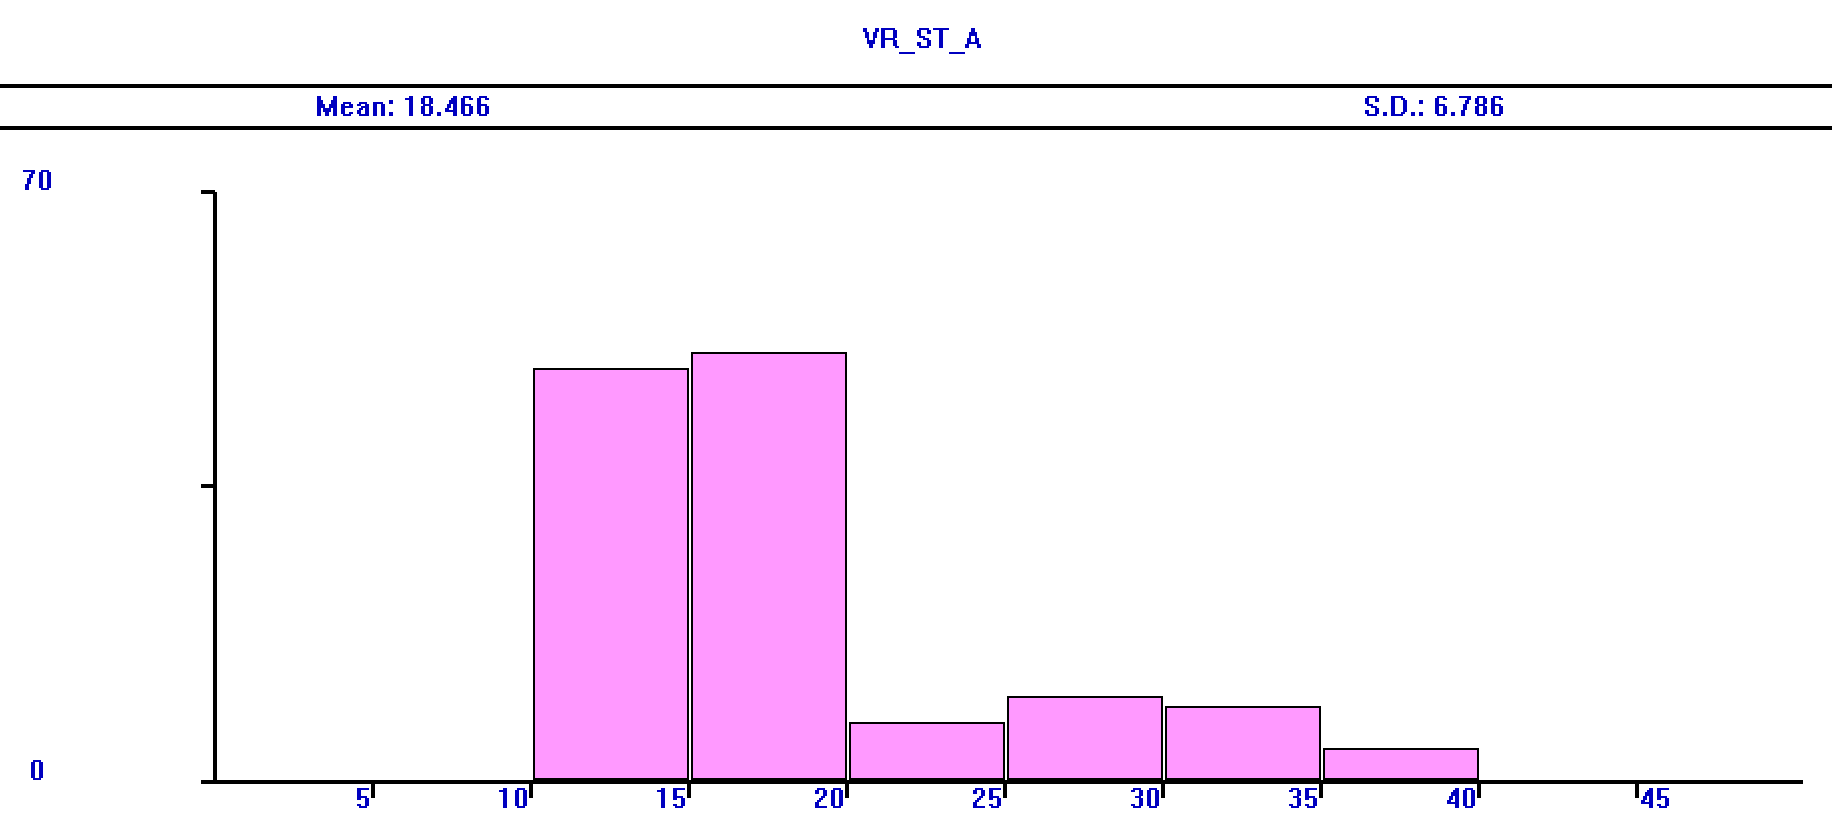
\includegraphics[width=0.8\linewidth]{pic/histogram_1}
  \caption{Гистограмма, построенная на основе данных о времени \\
    простоя станка типа~A}
  \label{pic:histogram_1}
\end{figure}

\begin{figure}[h!]
  \centering
  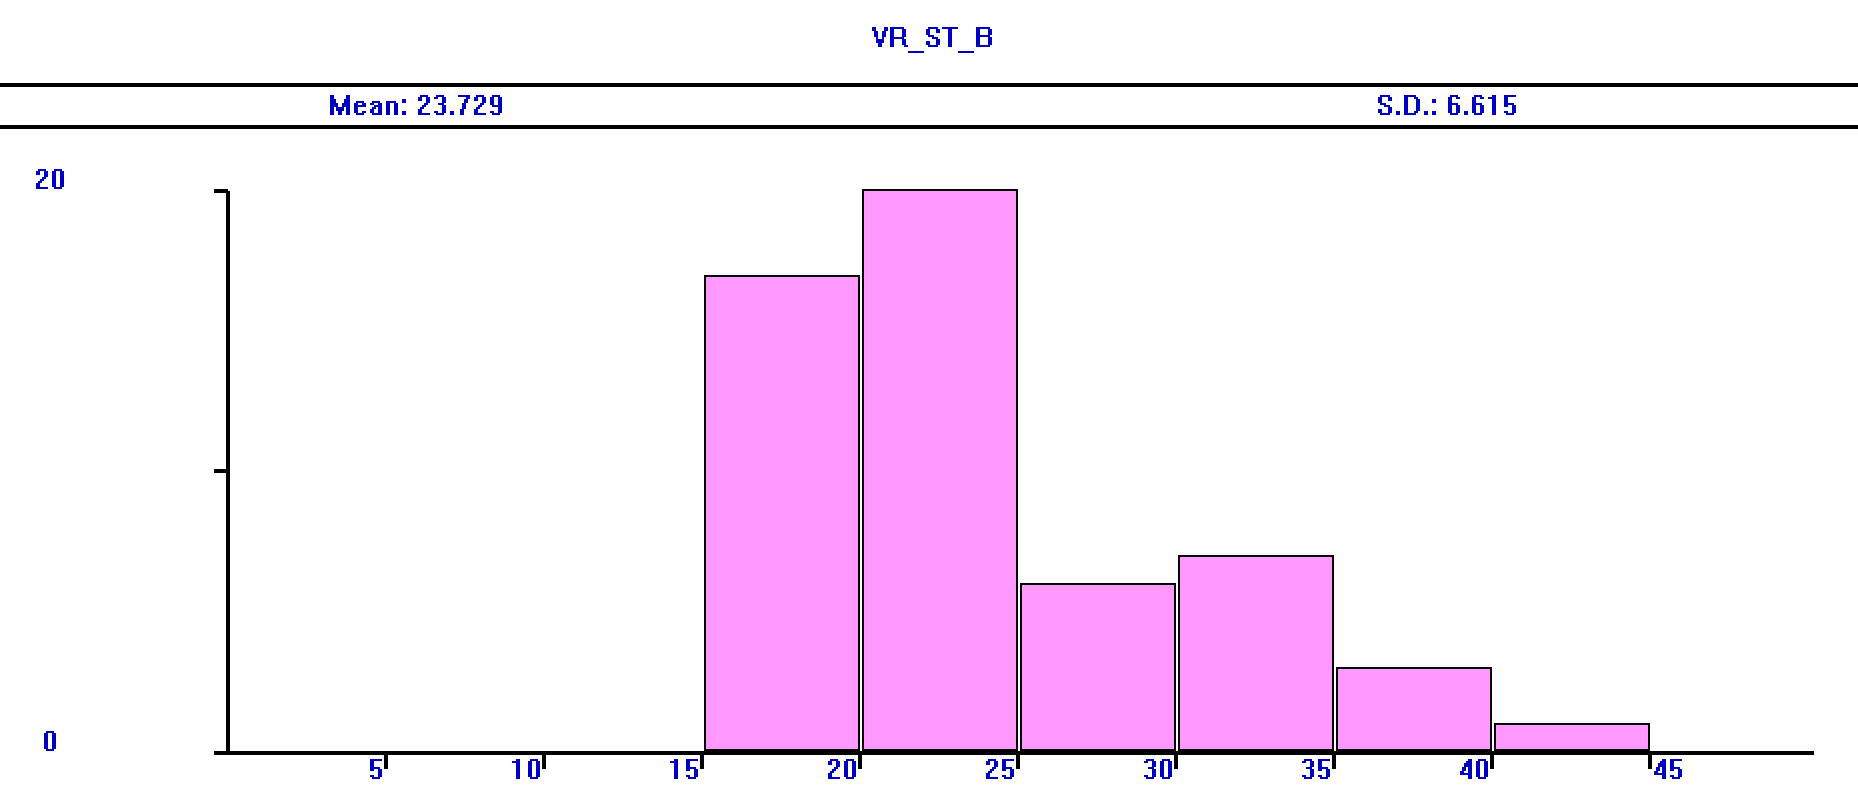
\includegraphics[width=0.8\linewidth]{pic/histogram_2}
  \caption{Гистограмма, построенная на основе данных о времени \\
    простоя станка типа~B}
  \label{pic:histogram_2}
\end{figure}

\newpage
